\chapter{An Approach for Reproducible Analysis}

\begin{center}
  \textit{If you're doing an experiment, you should report everything that 
    you think might make it invalid - not only what you think is right about it; 
    other causes that could possibly explain your results; and things you 
    thought of that you've eliminated by some other experiment, and how they 
    worked - to make sure the other fellow can tell they have been eliminated.}

 - Richard Feynman
\end{center}



\section{NMR data analysis is irreproducible}
Successful achievement of a reproducible NMR study requires reproducibility at 
each stage of the process.  First, the protocol for expressing, purifying, and 
preparing the sample of interest for experiments inside the NMR spectrometer 
must be reproducible, as well as the exact experimental conditions, 
spectrometer, pulse sequences and collection times used to collect the 
time-domain data must be captured.  Second, the software, platform, functions, 
and parameterizations for spectral processing stage must be captured.  
Third, both the computational results of peak-picking, GSS construction,
GSS assignment, and resonance assignment as well as any manual changes, 
along with the associated deductive process of reasoning, must be captured.  
Fourth, analysis and assignment of NOESY spectra, structure calculation, 
stereospecific resonance assignment and structure refinement must be captured.  
This last stage may also include computational as well as manual analysis 
components.  

This work will focus on reproducibility of the third and fourth stages, 
spectral analysis and structure determination.  Unfortunately, according to 
the definition of reproducible NMR given above, these stages are irreproducible.

Much work has been done to capture additional data from the assignment process.  
The CCPNMR effort, including the significant projects of CCPN Analysis and the 
CCPN data model \cite{ccpn}, captures a significant portion of final data.
Other significant efforts include SPINS \cite{baran2006spins}, 
Sesame \cite{sesame}, and the NESG \cite{nesg2005nmr}.  
However, much of the previous 
work in this area has focused on project management rather than reproducibility.
While SPINS is effective at capturing intermediate and final results, it is 
only intended for use on primary data files -- it is not designed to capture 
the key meta data mentioned above.  Sesame is capable of project management; 
however, it is intended for use in high-throughput studies.  ELNs 
\cite{rubacha2011eln}, while effective at capturing experimental design and
data, are not designed to support in-depth analysis, nor are they intended
to interface with NMR tools.

While the need for integration of automation with occasional manual 
validation and editing has been recognized \cite{baran2006spins}, no 
current systems are capable of combining these features with full 
meta data capturing.  
What is still missing is an approach and tooling for collecting all the primary 
data and meta data of NMR spectral analysis and structure determination.  Much 
time and effort is expended in these stages, but the data is not recorded.  The 
result is that the final data sets deposited into the BMRB are incomplete.



NMR data analysis is irreproducible because insufficient information is
captured during the process.  
This chapter will outline the data involved in NMR, and then 
describe in more detail the missing data, its role and importance, 
then a model for capturing that data, and a strategy for using
the model during the analysis process.



\section{Missing data and its role in analysis}
% need to cover what the data is, how it plays a role in NMR analysis, 
% why it's important to capture
The key deficiencies causing irreproducibility are missing primary data and 
meta data.  These data are not modeled in the CCPN data model nor in the 
NMR-Star data dictionary, and therefore are not archived and disseminated.
Spectral analysis, including peak picking, GSS construction, GSS and resonance
typing, sequential GSS assignment, and sequence-specific GSS assignment is 
accomplished using a step-by-step process of deductive reasoning 
which is often augmented by computational tools.  The computational 
results may be subject to manual validation, correction, and extension
\cite{guerry2011automated}.  This section will explore the various types
of data involved.


\subsection{Deductive process of reasoning}
Manual modifications are performed using a process similar to deductive 
reasoning.  It follows a general pattern:
\begin{enumerate}
  \item identification: a feature of the data is identified as amenable to 
    interpretation.  For example, the feature may be a false negative (such as 
    a signal peak misclassified as noise by the automated peak-picker), a false 
    positive (such as an artifactual peak misclassified as signal), or an 
    ambiguity (such as overlapped GSSs, causing clustering algorithms to fail).
  \item pattern recognition: the spectroscopist identifies a potential method 
    for interpreting the feature based on his/her domain knowledge of NMR and 
    experience with interpretation of previous data sets.  For example, such 
    methods may take the form of deductive rules:  if <the data matches a 
    certain pattern>, then <it could be interpreted a certain way>. 
  \item application of the rule to the data feature.  The chosen rule is 
    applied, and the result of the interpretation is included back into the 
    data set.  The result may now be used to drive further deductions.
  \item repeat -- go to step 1 to identify features for further interpretations
    This method is a form of iterative, sequential deduction.  The key components 
    are the ordered series of steps, the state of the data before and after each 
    step, and the deductive rules used to make interpretations at each step.  
    In addition, it should be noted that the final data set can not be 
    regenerated using automated tools alone if there are any manual 
    modifications made to tool output.
\end{enumerate}

The information describing the deductive process of reasoning employed in 
manually interpreting a feature of the primary data is not captured, although
it is important because it provides the explanation 
of why something was done.

Each deductive reason is an embodiment of NMR-specific knowledge of how to 
interpret a data feature.  In general, a deductive rule requires an input, 
produces an output, and has an intuitive justification for its action.
% TODO example

Application of these rules provides a rationale for manual modifications.  The
rationale is a justification that the change modification is correct, as
well as an indication of why the change was made.  Therefore, capturing the
deductive rules employed enables verification of the veracity of modifications. 
It also facilitates knowledge transfer, both in the contexts of collaboration
and teaching, by providing a meaningful annotation (with reference to the
domain of NMR) for actions taken.


\subsection{Intermediate results: deductive contexts}
When the output of a computational tool, whether peak-picking, GSS construction, 
or sequence-specific GSS assignment, is modified to correct mistakes,
a discrepancy is introduced between the output of the tool 
given the input and a suitable parameterization, and the final data set. 
This indicates that the final results are not the output of a single 
replicable step, but rather of a series of steps of refinement and 
modification.  Thus, new data sets are implicitly generated from the previous
one during the analysis process after every modification, whether manual or automated.
The application of a deductive rule to modify the data set is sensitive to
the current state of the data set -- in other words, the validity of the 
use of a given rule, as well as its effect, depends on the exact state of
the data set.  Therefore, it is important to record the data context when
applying a deductive rule.  The rectifies the discrepancy between automated
tool output and the final data set.  Unfortunately, this data is not recorded.

With respect to reproducibility, the importance of capturing intermediates is 
due to the dependence of deductions on context: without knowing the context, 
it is impossible to evaluate the correctness, confidence, and alternative 
interpretations of a deduction.  In standard approaches to analysis, the 
contexts are not captured; they are implicit.  By making the contexts 
explicit, it becomes possible not only to fully recapitulate the process of 
analysis, but also to employ error detection and correction strategies by 
analysis of deductions and their contexts.  An interesting side-effect of 
capturing contexts is that analysis can be restarted in the middle, by 
selecting an appropriate context and applying a different deduction.

% TODO
% come up with a simple example that demonstrates: 
%   1) the dependence of deductive ability on context
%   2) the concept and utility of multiple snapshots
%   3) the concept and utility of tracking logical dependencies

Furthermore, during manual analysis and modification of results, when the 
state of the data is continually being modified and improved, the analyses
which may be made are dependent upon the data context.
For example, assignment of a GSS to a residue may allow a further 
unambiguous assignment of a different GSS to a residue (an assignment 
which previously would have been ambiguous) by eliminating one of two 
assignment possibilities based on matching amino acid type.
% TODO explain better, provide an example
Implicit in the sequence of data sets are logical dependencies of derived
data upon features of the previous data set: the context of each deduction
is important, because the exact context determines what deductions may be
made and the confidence level of each deduction. 

% TODO I need to discuss what the intermediate results need to do
%   i.e. they need to make the process recapitulatable
%   and this is done by capturing the contexts


\subsection{Extraneous results}
Standard approaches use the 
assumption that all peaks are true signal, with no provision for storing peaks 
determined to be processing artifacts or noise.  Such spurious peaks are simply 
deleted and do not show up in the final results.  This is a problem because the 
fact that a peak was found, and later interpreted as noise does not show up in 
the final data set.  The same problem applies to GSSs that are found 
but can not be assigned to any residue of the sample of interest, or are 
believed to correspond to atoms of a contaminant.  Such GSSs should 
be represented in the final data set.

During analysis, some portion of the positive results are not of direct interest
to the final answer.  Not only peaks, but also resonances and GSSs are included.
The positive results include both false positives, caused by noise or
artifacts, and true positives, caused by contaminants.

Although not of direct interest, such extraneous results play a role in 
the process of analysis: as was covered earlier, when making a manual
modification, a deductive rule is applied to a context (data set).  Changing 
the context affects which rules apply and what deductions are made; 
therefore, as a part of the context, extraneous results matter during analysis. 
If incorrectly identified or left unrecognized, extraneous features can
lead to incorrect peak picking, chemical shift assignments, GSSs, and GSS
assignments.

A further benefit of capturing extraneous results is the ability to distinguish
between identifying a data feature and interpreting it.  In other words, peaks
picked during peak picking are treated as positives, this is the "identification"
phase; in the later "interpretation" phase, these peaks are separated into
false positives and true positives.  This allows rectification of the 
discrepancies between uncorrected computational results and the final,
deposited results as well as marking potentially suspicious results for 
future perusal.  It should also be noted that picking a peak, then
interpreting it as extraneous and discarding it is typically not reported in
final data sets, despite containing important information.
There is a balance between false positives and false negatives \cite{pine};
false negatives are more undesirable \cite{pine, saga, guntert2009automated},
and capturing extraneous results helps to avoid this tradeoff: by reducing
the cost of a false positive, tools are free to focus on avoiding false
negatives.

The process of separating positives into false and true is prone to 
introducing bias; by keeping and reporting the initial results, such bias
can be estimated.  This is not possible if the extraneous results are not
reported, and also allows the feature identification phase to proceed
without bias, since error correction will be applied at a later stage. 
By providing additional context, it may be possible to estimate the quality 
of an analysis, where errors may be most likely found in the borderline 
cases; it will also help assigning confidence levels to datums by not.
Additional quality measures enabled include the number of peaks found by the
peak-picker, the number of false positives, the number of peaks assigned to
GSSs, and the number of GSSs assigned to residues.  It may also be possible
to estimate contamination, incompleteness and overcompleteness, overfitting, 
and consistency.


\subsection{Notes: incompletions, uncertainties, ambiguities}
During the course of data analysis, it is often the case that odd, ambiguous,
abnormal, or otherwise unexpected situations noticed during analysis
\cite{nuseibeh2000inconsistency}.  
% TODO however, no record is made, blah blah .... these are valuable b/c blah blah
As notes indicate the deficiencies and 
potential problems present in a data set, they are valuable to future 
perusers as they highlight how a data set is flawed and how it can be improved.

Due to the difficulties inherent in data analysis, situations are reached
in which the interpretation of a specific feature is problematic:
\begin{itemize}
  \item uncertain or impossible.  The evidence for a particular deduction 
    is not solid.
  \item ambiguous.  Multiple interpretations of a feature are consistent
    with the data and satisfy the constraints.  It is not possible to choose
    between them.
  \item inconsistent.  The data set is in an inconsistent state, or a 
    deduction would leave it in an inconsistent state.
\end{itemize}
A simple example is non-stereospecific sidechain proton assignments: 
a residue such as a Histidine or Lysine which has two beta protons will 
often give rise to two resonances, one for each beta proton; however, 
without additional information, it is impossible to assign a resonance to
a specific atom.  A related example is caused by the two delta and epsilon
protons in Phenylalanine and Tyrosine aromatic sidechains; the two resonances,
even if distinguishable, can not be uniquely assigned to atoms.  In both
cases, the ambiguity is resolvable through the use of additional information;
however, before that additional information is provided, it is useful to be
able to store what is known -- that there are two peaks, each of which 
corresonds to one atom, but exactly which is unsure -- as an indication to
future analysis or perusal that a problem has been identified but not yet
solved.

% TODO add a picture
Correctly identifying and characterizing peaks in the presence of significant
amounts of overlap is a notoriously difficult problem \cite{guerry2011automated}.
The number, position, and intensity of peaks become distorted by the overlap.
In such a case, it may not initially be possible to fully and correctly
resolve the overlap (although later information from additional spectra, such
as a higher-dimensional spectrum in which the additional dimension removes
the overlap, may resolve the problem); a note explaining that overlap is
suspected and that the characterizations may be in error points this out.

% TODO add a picture
Building unambiguous and complete sequential GSS assignments is complicated 
when multiple GSSs have the same or nearly the same chemical shift values
for resonances which are or potentially may be assigned to CA, CB, CO, or the
corresponding (i-1) atoms.  Leaving a note in the data set describing what
the ambiguity is ensures that this information is not lost, and is clearly
marked for re-analysis when more data becomes available.
% TODO make sure I don't describe the solution in this section -- rather, it should be about the problem !!


\section{A Model for Reproducible NMR}

A data model is a means of specifying the structure of information  
\cite{codd1970relational}.  This
information may be used as inputs and outputs for computational tools, or
it may be archived and available for reference use.  Data models are useful
because they provide a formal specification of the structure, which enables
unambiguous, correct, and automated use of data.  Data models are
abstract specifications; they must be implemented in source code in order
to become a usable artifact.

This section will cover a data model for reproducibility.  Once a data
model exists, it can be implemented as part of a software program that
facilitates reproducible data analysis, as will be covered in a later 
chapter.  The core of this data model is formed by the BMRB \cite{bmrb}
and CCPN \cite{ccpn} data models.  These models are then extended with
several additional data types and properties in order to enable 
reproducibility.


\subsection{Deductive reasoning}
When a data feature is interpreted, a deductive rule is used to provide
the result, given the input.  In order to support the capture of this data, 
a model both for the application of a rule to a data set, and for the rules
themselves, was created.  The rules are modeled as an extensible library of 
commonly used deductive reasons.  Modeling the rules as an enumerated library 
enables quick and easy use.  During analysis, one or more rules are applied to 
make a deduction.  This is shown in Figure \ref{deduction_model}.

The content of the deductive rule library is based on 
established practices during data analysis \cite{guerry2011automated, hncacb,
hnco, cbcaconh, hbhaconh, picky, xeasy, sparky, ccpn}.  For each rule, 
a meaningful name, an explanation of the rule's meaning, its intended use,
its intended result, and examples was collected.

A library of commonly used deductive reasons is presented in Appendix 
\ref{sec_library}.



\subsection{Intermediate results}
The general outline of the solution is a model of the process of data analysis,
consisting of a sequence of snapshots of the data set, taken at carefully chosen 
moments during analysis, which show the full process of analysis by capturing
all changes.  Each snapshot -- other than the first -- contains a link to
the previous snapshot, as well as a set of data differences.  The differences
between snapshots provide the key value of this solution: they explicitly
show how the data set is changed over time.
Associated with each snapshot is a small amount of meta data to help describe
the snapshot, including a timestamp, author information, and a deductive
annotation, which describes the "why" of the changes and will be covered in
the next section.

The core of the strategy is based on that used by Version Control System (VCS) 
software tools \cite{vcs_concepts, hinsen2009vcs}, which are commonly 
applied for managing source code of 
software projects \cite{loeliger2012git, cvs, svn}.
These tools were originally implemented in order to manage the change in 
source code over time, while retaining the ability to easily inspect past 
states of the code.  It was found that application of such tools led to 
large increases in productivity, robustness, correctness, and reduced 
faults \cite{fischer2003vcs}.

While the general solution is adapted from version control software, in order
to effectively capture intermediate NMR data sets, such that the process of
analysis is clear and understandable, the solution must be augmented to fit
the specific needs of the NMR domain.
In other words, capturing meaningful intermediate snapshots is challenging; it 
is not sufficient to capture them indiscriminately.  If snapshots are captured 
too infrequently, the situtation is not significantly different from current 
practices: the analysis process will not be reproducible.  If too many snapshots
are captured, reconstructing the logical dependencies will not be possible;
in addition, the valuable information may be difficult to identify compared to
the large amounts of useless information.  A third potential problem is 
collecting snapshots indiscriminately -- i.e. not in a manner that corresponds
to the actual process employed.  This, too, prevents later use of the 
intermediate data because the process has not been correctly captured.

Therefore, there are several principles of intermediate data collection which
must be observed in order to create a useful data set.  These principles help
to ensure that snapshots are created neither too often nor too rarely, and
that they are useful for future perusal:
\begin{itemize}
  \item time.
    Snapshots should be taken often enough that all modifications are captured.
    For example, when peaks are initially picked by an automated tool, and then 
    modified (perhaps sorting them into signal, noise, and artifact classifications)
    by manual adjustment, a snapshot must be taken immediately after the automated
    peak picker is run, and before any modifications are made.  When additional
    modifications are made, it is again necessary to take another snapshot before
    these changes, in order to capture the previous state of the data set -- which
    is otherwise lost if this is not done.
  \item content.
    Each snapshot should have a clear and simple focus on analyzing a single
    feature or performing a single type of interpretation.  For example, a snapshot
    should not include changes both to resonance typing and to peak lists if those
    changes are not inter-dependent.  % this ensure that logical dependencies are recoverable ? ... 
  \item cohesion.
    Similarly to the previous point, changes which are inter-dependent belong in
    the same snapshot.  For example, when assigning GSSs sequentially, assume there
    are two potentially matching GSSs based on CA and CB resonances, which however
    have not been specifically assigned i/i-1.  If one GSS is determined to be the
    first, and the other the second, then the CA(i), CA(i-1), CB(i), and CB(i-1)
    assignments of the resonances in both spin systems are determined.  These 
    changes all naturally belong in a single snapshot, since they are logically 
    co-dependent.
  \item logical dependencies must be recoverable.
    The previous two points enable recovery of deductive, logical dependencies.  
    The sequential process of deduction is the core of manual analysis, and 
    therefore it is important to capture it clearly.  This means that the 
    dependencies must be reconstructable from the sequence of intermediate data 
    sets.
\end{itemize}

% devote more space to discussing diffs/comparisons, logical dependencies
%   what, why, and how.  
%   also, how the VCS-based solution supports these goals
The primary goal of capturing intermediate data sets is to 
facilitate reproducibility by modeling and saving the process of analysis.  
A system which does so by capturing a sequence of snapshots of the data set 
at intermediate timepoints meets the requirements for reproducibility.
First, such a system is able to correctly recapitulate the changes over time
due to manual and automated analysis.  For example,
if an automated peak picker were used on a spectrum, and then the results
manually verified and corrected, if snapshots were taken at the appropriate
moments, the sequence of snapshots would show both the complete results of
the automated tool, as well as every manual change made.
% TODO should I say more here?
Second, by capturing the full context of each modification, the logical and 
temporal dependencies between various features of the data set are trackable.
% TODO what? the following doesn't make much sense
Additionally, capturing multiple intermediates allows rich comparisons to be made 
between snapshots.  These comparisons, combined with the deductive annotations,
indicate the changes made with each specific deductive reason. 


\subsection{Extraneous results}
Our approach is to allow any number of peaks and GSSs, and to 
augment them with additional data fields which distinguish between signal, 
noise, contaminants, etc.  This allows one to make a critical distinction 
between: 1) finding/recording a peak based purely on characteristics of 
the spectrum such as volume, height, relative height compared to noise, 
lineshape, and linewidth, and 2) interpreting a peak as signal, noise, 
etc. (and the same for GSSs).  Even peaks and GSSs for 
which no analysis is made can be kept in the data set without encumbering 
assignment of true peaks and GSSs.

To model extraneous results, the BMRB and CCPN models \cite{bmrb, ccpn}
were extended to support additional fields which distinguished between 
extraneous and primary data.
This applies to peaks, resonances, and GSSs.
The general approach for using this model is to never directly delete
a peak, resonance, or GSS, but rather to mark it as extraneous by modifying
its associated category from 'signal' to 'artifact', 'noise', 'contaminant'
etc.

For example, while using an interactive spectral analysis such as Sparky or
CCPN Analysis \cite{sparky, ccpn} for peak picking a spectrum, it is common
to run the automated, built-in peak picker and then to manually correct the
results by deleting some peaks and adding new ones.  This approach would
work differently; peaks would not be deleted.  If the category of each of the
peaks initially picked by the automated tool were 'signal', then the task of
the user would be to correct all of the categories for peaks which were 
determined to be signal or noise; note that these peaks would not be deleted
from the list.  They would remain in the list but with a different category
tag that would differentiate them from signal peaks.

A further category of extraneous data is peaks from amino acid sidechains; 
it is presented in Tables \ref{nhsqc_peaktypes}, \ref{hnco_peaktypes}, 
\ref{hncacb_peaktypes}, \ref{hbhaconh_peaktypes}, \ref{cconh_peaktypes}, and
\ref{hcconh_peaktypes}.  While most of the
peaks in these experiments correspond to backbone covalently bond atom groups, 
and are used for backbone sequential assignments, many sidechain GSSs are
visible as well.  Although these peaks are often ignored, they do contain
useful information.  They also can confound analysis if they are not properly
recognized as sidechain peaks.  Lastly, their presence is surprising to 
newcomers to the analysis process, as they are typically not explicitly 
recognized as part of the standard experiments.

% TODO a pictoral representation of this model
% TODO examples
% TODO 
% CCPN peak pick as initial peak list, then corrections I made as peak list 
%   where each peak has additional fields


\subsection{Notes}
The key idea is, given the inevitability of such problems during data
analysis, to create facilities for explicitly recognizing, discussing, 
and handling such problems \cite{robillard2007concerns}. 
Several strategies for such an approach 
are covered in \cite{nuseibeh2000inconsistency} including deferral of the
problem while flagging it for later follow-up.

To model notes, the BMRB and CCPN models \cite{bmrb, ccpn} were extended
to support an additional data type: a note.  A note can refer to one or more
other feature of the data set, and also includes a textual description of
the nature of the problem, as well as an indication of how the problem might
be resolved (although that is optional).  As the purpose of a note is to
explicitly indicate known deficiencies, incompletions, or uncertainties in 
the data set, wherever and whatever they may be, this approach is able to do
so.
% TODO a pictoral representation of this model
% TODO example: odd feature in data, unable to resolve

Enabling the representation of such data has similarities to the probabilistic
approach applied by PINE \cite{pine} to great effect.  
PINE deals with the innate uncertainty of data 
analysis by resolving the tradeoff between false positives and false 
negatives through association of a probabilistic confidence metric with each
feature interpretation; low confidence values are used as evidence that an
interpretation is suspicious and needs additional verification or data.
In a complementary approach, capturing notes of analysis issues also 
resolves the tradeoff for manual analysis, by enabling the association of
an explanatory or warning message with suspected low-quality deductions.
In addition, the message may contain more information than a scalar: it may
necessarily refer to multiple conflicting pieces of the data set in the case
of a contradiction.



\section{An implementation of the model}
A software implementation of this model was created as an extension to the
popular assignment program Sparky \cite{sparky}.  Sparky natively provides
facilities for spectral viewing, peak picking, spectral analysis and 
resonance assignment; the extension augments the native features with 
features which facilitate reproducibility: easy capturing of snapshots,
easy snapshot annotation with deductive reasoning, and easy capturing and
identification of extraneous peaks and GSSs.
The design, implementation, and use of this program is covered in 
detail in Section \ref{sec_sparky_extension}.



\section{Applying reproducible analysis: using the model}
This section presents some general advice for how to use the reproducibility
model effectively in practice.  It provides tips and suggestions, as well
as covering common problems and how they can be avoided.

\begin{itemize}
  \item one snapshot, one focus.  Keeping each snapshot focused on dealing
    with a single issue helps the process of analysis to remain understandable
    to later perusers.  This is because it makes the logical dependencies 
    more obvious; when a single snapshot contains many unrelated things, or
    is extensive enough that part of the snapshot depends on other parts, then
    it is no longer clear what the logical relationships are.  Keeping snapshots
    small and focused alleviates this issue.
  \item level of detail.  It is not necessary to exhaustively annotate every
    last single change; clearly, such an approach would be problematic because
    it would require far too much time and effort on the part of its users.
    Rather, the value of this reproducible approach is to clearly indicate 
    major issues and modifications.  The more important and the more time and
    brain power went into making a deduction, the more annotation it typically
    deserves -- in other words, a complicated deduction requires a complicated
    justification.  On the other hand, if multiple peaks are quickly and
    straightforwardly identified as artifactual with a minimum of effort, 
    only a bare minimum of annotation is needed; the deduction does not become
    clearer with additional annotation.
  \item apply the correct rule(s).
  \item record uncertainty and resolution.  When in doubt or difficulty 
    during analysis, record all information pertaining to the issues, whether
    as a note or extraneous data.  Even if the problem is easily or quickly
    solved, describing it creates a record of that problem which is valuable
    for later perusal.  Trends over such a record help to indicate more 
    large-scale problems, as well as illuminating troublesome spots for
    collaborators and learners.
\end{itemize}
   
% maybe talk about the culture of the lab notebook?
% could this belong in its own chapter?
% or in the software chapter, or in the 'reproducible data sets' chapter?


\section{Future directions}
The deductive library is not complete -- it does not include deductions for
every single possible analysis or interpretation which may be performed on
NMR data.  Examples include residual dipolar couplings, hydrogen bonds,
and pseudocontact shift restraints.  However, the library is extensible: it
can be easily augmented with new deductive reasons.  This is important because
even if the library were complete today, it would likely still need to be
extended in the near future to deal with new types of analysis and new data
types.  Thus, the strength of the approach that has been presented here, and
its corresponding model, is that the approach is orthogonal to the specific
datatype under analysis, which allows the library to be extended as necessary.

A further source of incompleteness is that of tools such as Sparta+, Cheshire, 
Shifty, CS-Rosetta, and ShiftX2 \cite{sparta+, cheshire, shiftx2, cs-rosetta, shifty}.
These tools enable new interconnections between various stages of the analysis
process (see Table \ref{data_connections} and Figure \ref{process_timeline}), 
creating possibilities for skipping steps or going backwards in the
process in order to verify that results are consistent with expectations.  
Effective use of these tools employs several useful deductive rules, similarly
to manual analysis.  Again, as the deductive library is extensible, it would be
straightforward to add deductive reasons for incorporating the results of these
tools into the analysis process.


\section{Discussion}
By collecting reproducible data sets, the true information content used in
NMR spectroscopy is made explicit and visible.  This is analogous to how lab
notebooks are intended to be used in wet-lab work: as a means of recording
the crucial details describing how an experiment was done, so that the procedure
can be shared with and improved upon by others.  A key difference, however, is
that while lab notebooks have been in use for several centuries, the culture
of reproducibility of digital analysis is still in its infancy: we do not yet
have much experience with the what, how, and why of reproducibility in 
electronic media.

The first step is to define the lost data and a model for it.
Then the model must be applied in practice, and its correct use taught.
By extending standard existing models, the barrier to entry is greatly reduced,
and instead of requiring an abrupt and drastic change in the workflows of those
already using the standard models \cite{bmrb, ccpn}, the change to reproducible
analysis can be incremental and gradual.  This should help adoption.

Not only will such data sets make the process explicit, they will also help
make biases explicit.  It is possible that different research groups and
different analysis techniques have different innate biases; it is quite likely
that such biases will become obvious through the collection of these full data
sets.  Each bias will represent an opportunity for learning and for improving
the quality of analysis.

A natural question to ask of the approach is whether it is able to deal with 
the various strategies employed in practice by NMR spectroscopists around the
world.  Is the library of deductive reasoning sufficient for all use cases?
While it is not possible to prove that the approach is universal, it is not
necessary to do so.  Rather, it is important to identify the principles of
NMR data analysis, and embody them into the library.  Furthermore, this risk
of non-universality has been mitigated by the extensibility of the library:
although as much was included as was reasonably possible to identify, if 
a deficiency is found in the library, it can easily be rectified by extending
it with an additional deductive reason.


% figures
\clearpage
\section{Figures}

\begin{figure}[h]
  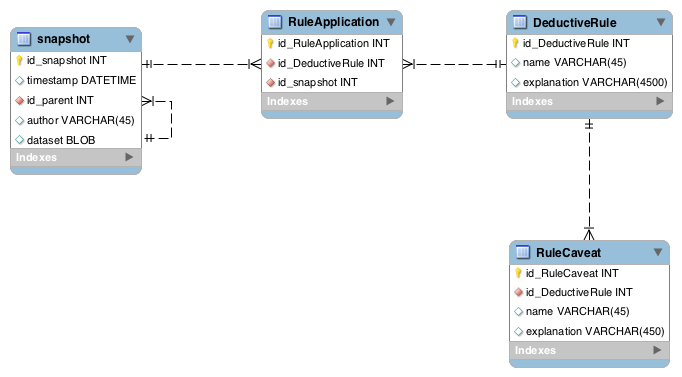
\includegraphics[scale=0.5]{figures/deduction_model}
  \caption{A relational model of a snapshot and deductions.}
  \label{deduction_model}
\end{figure}

